\documentclass[12pt]{article}
\setlength{\parindent}{0pt}
\usepackage{relsize}
\title{Monocular Depth Estimation Using Object Scaling \\ \smaller{TEK5030 Project Report}}
\usepackage[final]{pdfpages}
\usepackage{amsmath}
\usepackage{graphicx}
\usepackage{float}
\author{Didrik Samdanger, Carlos Ankour Navarro, Bryan Walther}
\usepackage[utf8]{inputenc} 
\usepackage{listings}
\usepackage{xcolor}
\usepackage{amssymb}
\graphicspath{ {./Figures/} }
\renewcommand\arraystretch{1.2}

\definecolor{codegreen}{rgb}{0,0.6,0}
\definecolor{codegray}{rgb}{0.5,0.5,0.5}
\definecolor{codepurple}{rgb}{0.58,0,0.82}
\definecolor{backcolour}{rgb}{0.95,0.95,0.92}

\usepackage{hyperref}
\hypersetup{
    colorlinks,
    citecolor=black,
    filecolor=black,
    linkcolor=black,
    urlcolor=black
}

\lstdefinestyle{mystyle}{
    backgroundcolor=\color{backcolour},   
    commentstyle=\color{codegreen},
    keywordstyle=\color{magenta},
    numberstyle=\tiny\color{codegray},
    stringstyle=\color{codepurple},
    basicstyle=\ttfamily\footnotesize,
    breakatwhitespace=false,         
    breaklines=true,                 
    captionpos=b,                    
    keepspaces=true,                 
    numbers=left,                    
    numbersep=5pt,                  
    showspaces=false,                
    showstringspaces=false,
    showtabs=false,                  
    tabsize=2
}

\lstset{style=mystyle}
\lstset{extendedchars=false}


\begin{document}
\maketitle

\section{Introduction}
While stereo and multi camera systems exist for obtaining depth of various points, these systems often are expensive and can be difficult to calibrate correctly. 
Different means of identifying depth for computers include using ranging sensors and stereo cameras to the focus of this project, digital estimation using a single RGB camera. Ranging sensors, such as LiDAR, tend to offer high accuracy metric point clouds at a very high cost. Stereo cameras tend to be shorter range, and with reduced accuracy compared to LiDAR, though can still be quite expensive. 
To reduce cost and complexity, a reasonable estimate could be created with a standard, readily available RGB camera and modern computer vision techniques.
Monocular depth estimation in computer vision is the problem of extracting depth information of a scene from single images captured by monocular cameras.
In contrast, monocular depth estimation is an ill-posed problem, since we attempt to infer depth information of a scene using only visual cues of a single image.
Most modern approaches to monocular depth estimation involves using large datasets with labeled images to train deep learning models, where the ground truth depth information for each sample is included in the training set.
A popular model that does this is MiDaS, which is trained on up to 12 different datasets, and predicts the relative depth map for a given image.
However, the predicted depth maps only offer depth information up to scale, meaning that we face the issue of scale-ambiguity.
Some work has been done on attempting to learn the absolute depth of a scene, a notable example being ZoeDepth.
ZoeDepth attempts to learn depth information while also maintaining the metric scale.
After testing ZoeDepth however, we find that the accuracy of the model in predicting the true scale is generally poor.
\\ \\
In this project we attempt to tackle the problem of scale-ambiguity in estimated depth-maps by leveraging prior knowledge of the real world geometry of the scene.
As a proof of concept, we apply this idea to traffic footage, where the goal is to get good distance estimates from a dash-camera to any object in the scene.


\section{Background}
The depth map received from a DNN model will either be relative, as in only saying which objects are perceived closer, or metric, meaning absolute distance from the camera sensor. Relative depth maps tend to be easier to train and offer more reliability in their results, while metric depth maps offer more useful data. \\

% Comparison of MiDaS and ZoeDepth


\section{Proposed Approach}
\begin{figure}[H]
    \centering
    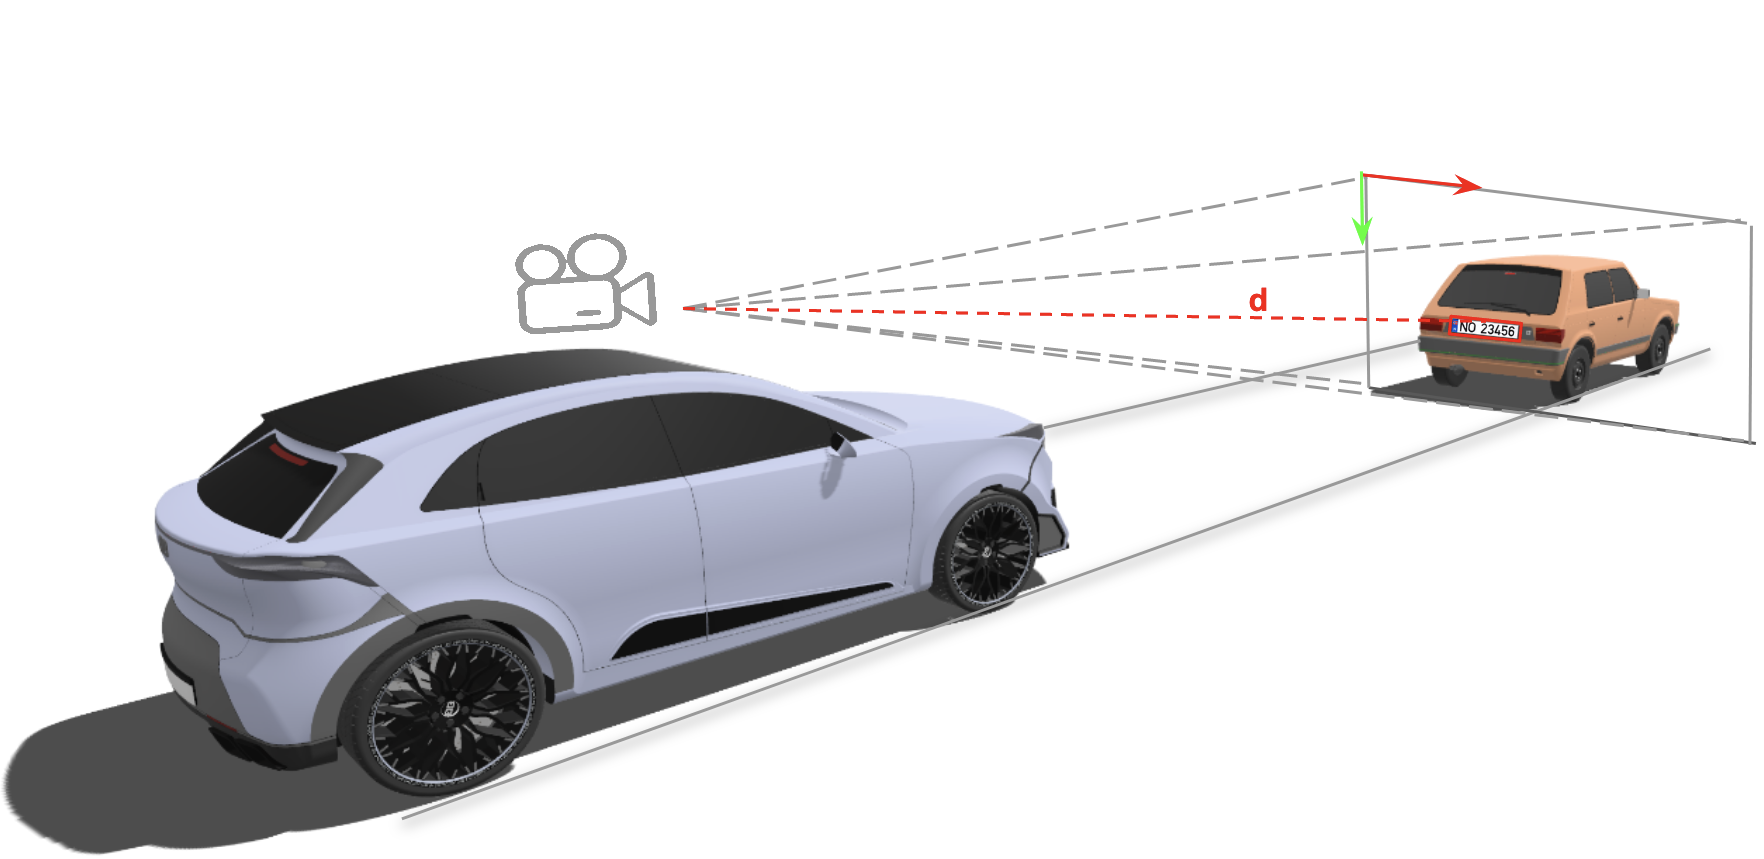
\includegraphics[width=1.0\textwidth]{illustration.png}
    \caption{Depth estimation of license plates }
    \label{fig:illustration}
\end{figure}

To achieve an improvement over the standard depth map estimations, our system would use the known dimensions of an object in frame to better estimate the distance to a given point, then apply that scaling to the rest of the depth map. License plates were chosen as they have standardized sizes and are guaranteed to be found on vehicles on the road. European Union style plates are $520\times110mm$, US style plates are $300\times150mm$ and Chinese style plates are $440\times140mm$. Automatic detection of which style of license plate as well as other dimensions for license plates will not be used in this project.\\

The algorithm would first use ZoeDepth to create a standard depth map across the image. Next vehicle regions of interest (ROIs) were identified and license plates would be detected from there. arbitrary targets would also be detected for later use. Given the known dimensions of the license plates, the distance from the camera to the vehicle could be calculated and a relationship between the calculated and estimated depth could be established. Lastly, a corrective scaling would be applied to the depth map and the targets identified earlier could be marked with a more accurate distance estimate.

\subsection{Depth maps using ZoeDepth}
In order to produce monocular depth map estimations, we turned to the popular DNN models from a repository called MiDaS \cite{ranftl2020robust}. MiDaS (v3.1) are a relative depth estimators trained on up to 12 different datasets. These datasets contain pairs of RGB images and depth maps from various scenes, taken with either stereo cameras or LIDAR sensors. MiDaS has a set of different pretrained weights and architectures to be used depending on certain desirable performance attributes, such as inference time and resolution. During testing of MiDaS´s perfomance for our application it quickly became clear that it is not necessarily straight forward to use.

\begin{figure}
    \centering
    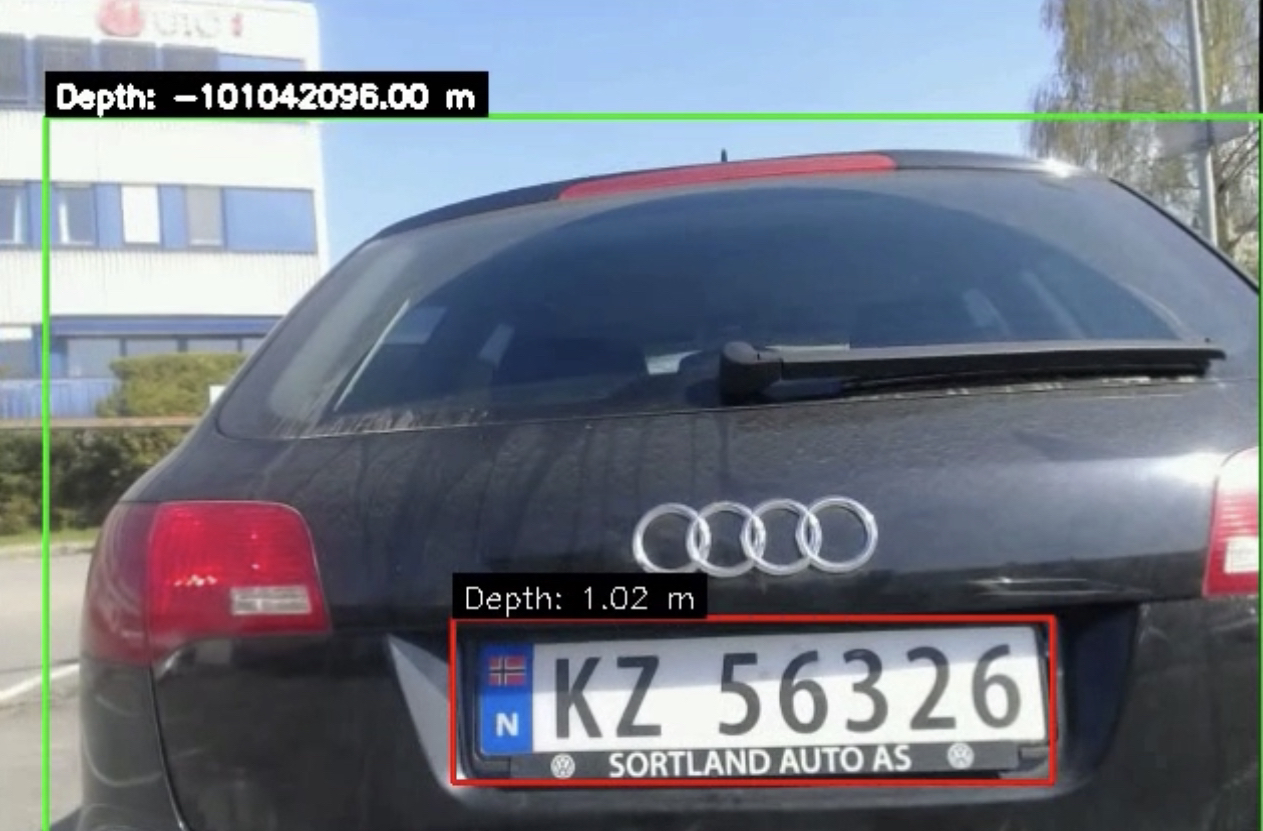
\includegraphics[width = 0.75\textwidth]{Figures/midas_problem.png}
    \caption{MiDaS results}
    \label{fig:midasProb}
\end{figure}

As seen in Fig.\ref{fig:midasProb}, the standard model for MiDaS

\subsection{License plate detection}
Initial tests intended to use machine learning to identify the vehicles, while traditional image manipulation methods would be used to identify the license plate size to keep the system as close to real time as possible. Car detection was handled by Cascade classifier, a lightweight machine learning matcher, and later with YOLOv4 and YOLOv5. The change did improve accuracy of detection and ROI selection, but at the cost of run time. \\

License plate detection was handled with canny edge detection and contour finding to locate shapes within the expected area of the vehicle ROI. These contours were then filtered based on the known dimensions of license plates. The plates could not be identified just by looking for contours that approximated four-sided polygons as lighting conditions and inconsistencies with cameras and videos tested meant that it was not reliable enough. Instead contour bounding boxes were used as best case approximations. As shown in Fig. \ref{fig:tradPlateDet}, the resulting detection rate was acceptable, though sometimes mistook brand badges and taillights as well. An attempt to improve accuracy was to implement a histogram to isolate selected ROIs that were primarily white backgrounds with black text, though this was not successfully implemented. Factors determined that limited this filters success were: resolution of the plate ROI, lighting conditions, and reverse lights on vehicles also returning similar values. Ultimately, it was decided that this project did not need real time operations and the license plate detection was also passed of to YOLOv5. \\

\begin{figure}
    \centering
    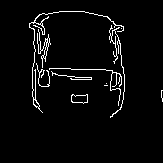
\includegraphics{Edges_screenshot_19.05.2023.png}
    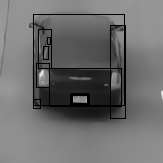
\includegraphics{Car ROI_screenshot_19.05.2023.png}
    \caption{Edge detection and Plate detection results}
    \label{fig:tradPlateDet}
\end{figure}

\subsection{Plate detection using YOLOv5}
The approach we went with for detecting the license plates in the scene was using YOLOv5 for the detection of the vehicles and ROI detection of license plates.
\\ \\
We used two separate weights for the detection in the algorithm.
For the detection of the vehicles as well as pedestrians we used the pre-trained weights from Ultralitics, which is trained on the COCO dataset.
For detecting the license plates, we used weights that were fine tuned on a dataset containing license plates from various different countries.
\\ \\
We first detect the vehicles in the scene as well as any other object in traffic that we want to know the distance from. The objects could be pedestrians, traffic lights, traffic signs, etc.
Once we have the vehicle bounding boxes, we do region of interest detection for the license plate within the bounding box of the vehicle. This is done for all the vehicle detections that we have per frame.
\begin{figure}[H]
    \centering
    \includegraphics[scale=0.3]{Figures/cropped_images.png}
    \caption{Cropped vehicle and license plate detections}
    \label{fig:my_label}
\end{figure}

% The final approach involved two weights:
%   - One for detecting vehicles and general objects in traffic
%   - One finetuned on a license plate dataset to detect the plate within the bounding box of the vehcile
% We then relate the license plate detections of the vehicle bounding box to the original image to get the (x, y, w, h) of the box relative to the original frame
% We end up with a collection of plates with known image width and height that can be used for the depth calculation.

\subsection{Depth Calculation}

\begin{equation}\label{eq:avgDepth}
    d = \frac{depth_{width} + depth_{height}}{2}
\end{equation}
\begin{equation}\label{eg:depthWidth}
    depth_{width} = \frac{focalLengthX * plateWidth}{plateWidthPx}
\end{equation}
\begin{equation}\label{eg:depthHeight}
    depth_{height} = \frac{focalLengthY * plateHeight}{plateHeightPx}
\end{equation}

% Mention how we assign the calculated depth to all the pixels belonging to the plate
% We then end up with an array of [(x, y, z)] which contains the depth for a set of pixels belonging to the detected plates

\subsection{Depth Correction}
Least squares method
% We keep a record of all the previous scale factors
% Filtering based on outlier detection of the scale factor for each frame, given the last n scale factors
% When correcting we use the running average of the last n scale factors
% This made it more stable

\section{Results}

Early testing using the traditional image manipulation showed promise as seen in Fig. \ref{fig:tradPlateDist}. It should be noted that the video used in this example was recorded by an unknown camera and depths values based on an average FOV are not accurate. Future tests using YOLOv5 used a mix of calibrated camera with known values and unknown cameras to test real world cases.

\begin{figure}[H]
    \centering
    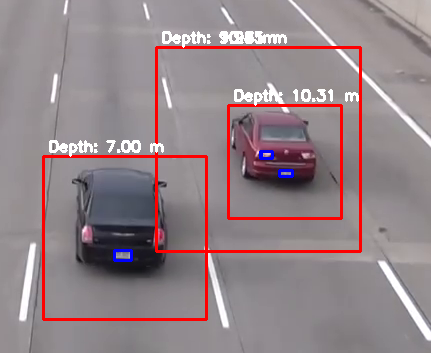
\includegraphics[scale=0.55]{RGB Screenshot from 2023-05-19 13-07-10.png}
    \caption{Early distance testing using traditional plate detection}
    \label{fig:tradPlateDist}
\end{figure}

\section{Discussion}
% Mention problems
%   - Its slow, lots of potential optimizations to be done
%   - Can be unstable with too many plate detection, could use good filtering of plate detections to remove bad detections.
%   - Potentially do some perspective correction to the plate detections.
% Mention use cases
%   - Generate a dense point cloud from the corrected depth maps per frame


\section{Conclusion}
Summary of key findings \\
Significance of object scaling for monocular depth estimation \\
Potential applications \\
Future work for this project would include optimization of the detection and depth estimation code. Real time operations would be the goal so systems such as this could be implemented onto unmand ground vehicles or other systems dependent of real time depth information. Expanding the scope to automatically detect license plate style would also improve accuracy over a wider range of environments. Additionally, other known objects could be added to improve depth estimation at various points.

\bibliographystyle{unsrt}%Used BibTeX style is unsrt
\bibliography{citations}
\end{document}
